\section{Ортонормированные базисы в $E$ и $V$}

$\mathbb{V}$ - это $E$ или $V$

\begin{shdef}
    \begin{definition}
        $x \perp y$, если $\langle x, y \rangle = 0$
    \end{definition}
    
    \begin{definition}
        $\mathbb{E}$ - базис в $\mathbb{V}$. \quad
        $\mathbb{E}$ - ОНБ, \ если $\langle e_{i}, e_{j} \rangle = \delta_{ij} = \begin{cases}
        1, & i = j \\
        0, & i \neq j \\
        \end{cases}$
    \end{definition}
\end{shdef}

\vspace{0.4cm}
\begin{shth}
    \begin{theorem}
        Если $a_{1}, \ldots, a_{k} \neq 0$ и $a_{i} \perp a_{j}, \ i \neq j,$ то это ЛНЗ система.
    \end{theorem}
\end{shth}

\begin{proof}
\leavevmode \newline

    От противного: Они ЛЗ $\Longrightarrow$ $\exists \ \alpha_{1}, \ldots, \alpha_{k}$ не все 0, что: 
\newline 

    $$(*) \ \alpha_{1} a_{1} + \ldots + \alpha_{k} a_{k} = 0$$
    Умножаем скалярно на $a_{1}$
    \newline
    
    $\Longrightarrow \alpha_{1} \langle a_{1}, a_{1} \rangle + \alpha_{2} \langle a_{2}, a_{1} \rangle + \ldots + \alpha_{k} \langle a_{k}, a_{1} \rangle = 0 \ \Longrightarrow \alpha_{1} = 0$
    \newline
    
    умножаем $(*)$ на $a_{2}$ и получаем, что $\alpha_{2} = 0$
    
    \
    
    $\Longrightarrow$ все $\alpha_{i} = 0 \ \Longrightarrow$ противоречие! 
\end{proof}
\vspace{0.6cm}

\begin{shth}
    \begin{theorem}
        (Ортогонализация по Шмидту)
        
        Пусть $\mathbb{V}$ - это $E$ или $V$, тогда:
        \begin{enumerate}
            \item ОНБ существует
            \item если ${(f_{1}, \ldots f_{n})}$ - базис в $\mathbb{V}$, то ОНБ можно построить по формуле:
            
            \[
            \begin{cases}
                \rho_{1} = f_{1}, & e_{1} = \frac{\rho_{1}}{\left\|\rho_{1}\right\|} \\
                \rho_{2} = f_{2} - \left(f_{2}, e_{1}\right) \cdot e_{1}, & e_{2} = \frac{\rho_{2}}{\left\|\rho_{2}\right\|} \\
                \vdots \\
                \rho_{n} = f_{n} - \left(f_{n}, e_{1}\right) \cdot e_{1} - \left(f_{n}, e_{2}\right) \cdot e_{2} \ldots - \left(f_{n}, e_{n-1}\right) \cdot e_{n-1}, & e_{n} = \frac{\rho_{n}}{\left\|\rho_{n}\right\|}
            \end{cases}
            \]
        \end{enumerate}
    \end{theorem}
\end{shth}

\clearpage
\begin{figure}[!h]
    \centering
    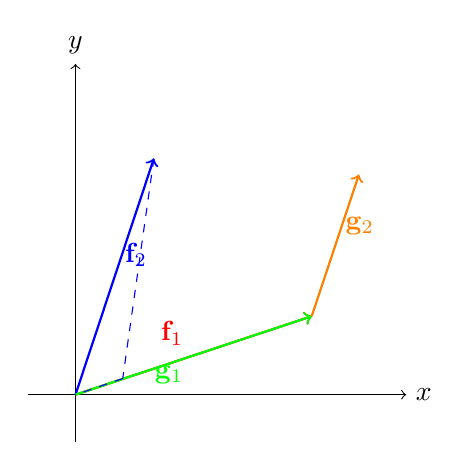
\begin{tikzpicture}[scale=1.2]
        % Оси координат
        \draw[->] (-0.5,0) -- (3.5,0) node[right] {$x$};
        \draw[->] (0,-0.5) -- (0,3.5) node[above] {$y$};
        
        % Исходные векторы
        \draw[thick, red, ->] (0,0) -- (2.5,0.83) node[midway, above left] {$\mathbf{f}_1$};
        \draw[thick, blue, ->] (0,0) -- (0.83,2.5) node[midway, above right] {$\mathbf{f}_2$};
        
        % Ортогонализованные векторы
        \draw[thick, green, ->] (0,0) -- (2.5,0.83) node[midway, below left] {$\mathbf{g}_1$};
        \draw[thick, orange, ->] (2.5,0.83) -- +(0.5,1.5) node[midway, above right] {$\mathbf{g}_2$};
        
        % Проекция v2 на u1
        \draw[dashed, blue] (0.83,2.5) -- (0.5,0.17);
        \draw[dashed, blue] (0.5,0.17) -- (0,0);
        
        % Подписи
    \end{tikzpicture}
    \caption{Визуализация ортогонализации по Шмидту}
    \label{fig:gram_schmidt}
\end{figure}

\vspace{0.4cm}

\begin{shth}
    \begin{lemma}
        \[ \forall k \in {\{1, \ldots, n \}} \quad g_{k} \in \mathcal{L}(f_{1}, \ldots f_{k}), \qquad g_{k} \neq 0 \]
    \end{lemma}
\end{shth}

\vspace{0.4cm}
\begin{proof}
    по индукции:
    
    \begin{enumerate}
    
    
        \item $ k = 1 \quad g_{1} = f_{1} \in \mathcal{L}(f_{1}), \quad f_{1} \neq 0$
        
        
        \item $k = m - 1  - \text{верно}, \; k = m ?$ 
        \nl

        $g_{m} = f_{m} - \inner{f_{m}}{e_{1}} \; e_{1} - \ldots - \inner{f_{m}}{e_{m-1}} \; e_{m-1} = f_{m} - \alpha_{1} g_{1} - \ldots - \alpha_{m-1} g_{m-1}$
        \nl
        
        Так как все $g_{i}$ линейно выражаются через $f_{1}, \ldots, f_{m-1}$
        \nl
        
        $\lra  f_{m} - \alpha_{1} g_{1} - \ldots - \alpha_{m-1} g_{m-1} = f_{m} - \beta_{1}f_{1} - \ldots \beta_{m-1}f_{m-1} \quad  \nl \lra g_{m} \in \mathcal{L}(f_{1}, \ldots, f_{m})$        
        \nl 
        
        если $g_{m} = 0 \lra f_{m} - \beta_{1}f_{1} - \ldots - \beta_{m-1}f_{m-1} = 0$
        \nl 
        
        Это нетривиальная линейная комбинация равная нулю $\\lra$ противоречие, \\nl так как $f_{1}, \\ldots, f_{m}$ - базис линейной оболочки $\\mathcal{L}(f_{1}, \\ldots, f_{m})$ 
    \end{enumerate}
\end{proof}

\clearpage

Теперь вернёмся к доказательству Теоремы 5.
\begin{proof}

Осталось доказать, что все оставшиеся векторы попарно ортогональны.

Докажем по индукции, что для всех \( k \in \{1, \ldots, n\} \) векторы \( e_1, e_2, \ldots, e_k \) образуют ортогональную систему.

\begin{enumerate}
    \item База индукции: \( k = 1 \).

    По построению \( e_1 = \frac{g_1}{\|g_1\|} \), где \(g_1 = f_1\). Так как \(\|e_1\| = 1\), то \( e_1 \) — единичный вектор.

    \item Предположим, что для некоторого \( k = m-1 \) векторы \( e_1, e_2, \ldots, e_{m-1} \) образуют ортогональную систему.

    \item Шаг индукции: \( k = m \).

    Покажем, что \( e_m \) ортогонален каждому из \( e_1, e_2, \ldots, e_{m-1} \).

    Рассмотрим вектор \( g_m \):
    \[
    g_m = f_m - \sum_{i=1}^{m-1} \langle f_m, e_i \rangle e_i
    \]
    По построению \( e_m = \frac{g_m}{\|g_m\|} \).

    Для любого \( j \in \{1, 2, \ldots, m-1\} \) вычислим скалярное произведение \( \langle e_m, e_j \rangle \):
    \[
    \langle e_m, e_j \rangle = \left\langle \frac{g_m}{\|g_m\|}, e_j \right\rangle = \frac{1}{\|g_m\|} \langle g_m, e_j \rangle
    \]
    Вычислим \( \langle g_m, e_j \rangle \):
    \[
    \langle g_m, e_j \rangle = \left\langle f_m - \sum_{i=1}^{m-1} \langle f_m, e_i \rangle e_i, e_j \right\rangle
    \]
    Раскроем скалярное произведение:
    \[
    \langle g_m, e_j \rangle = \langle f_m, e_j \rangle - \sum_{i=1}^{m-1} \langle f_m, e_i \rangle \langle e_i, e_j \rangle
    \]
    По предположению индукции \( e_1, e_2, \ldots, e_{m-1} \) ортогональны, поэтому \newline \( \langle e_i, e_j \rangle = 0 \) для \( i \neq j \).
    \nl 
    
    Следовательно,  $
    \langle g_m, e_j \rangle = \langle f_m, e_j \rangle - \langle f_m, e_j \rangle = 0 $
    \nl 
    
    
    Таким образом, $\langle e_m, e_j \rangle = \frac{1}{\|g_m\|} \cdot 0 = 0$. 
    Это означает, что \( e_m \) ортогонален каждому из \( e_1, e_2, \ldots, e_{m-1} \).
    \nl 

    Следовательно, векторы \( e_1, e_2, \ldots, e_m \) образуют ортогональную систему.
\end{enumerate}

\vspace{0.4cm}

Таким образом, по индукции мы доказали, что векторы \( e_1, e_2, \ldots, e_n \) образуют ортогональную систему. А так как все векторы \( e_i \) нормированы (\(\|e_i\| = 1\)), то система \( e_1, e_2, \ldots, e_n \) является ортонормированным базисом.

\end{proof}

\begin{shdef}
    \begin{definition}
    \leavevmode \\

        Ортогональная матрица — это квадратная матрица $A$ с вещественными      элементами, удовлетворяющая условию: 
        $$A^T A = A A^T = E$$
        \nl 

        Унитарная матрица — это квадратная матрица $U$ с комплексными элементами, удовлетворяющая условию: 
        $$U^* U = U U^* = E = \overline{A^T}$$
        \nl

        ($ U^* $ - транспонированная и комплексно-сопряженная матрица.)
    \end{definition}
\end{shdef}

\begin{shth}
\begin{theorem}
    \begin{enumerate}
    \leavevmode \nl 
    
        \item Пусть $\mathbb{V} = E$ — Евклидово пространство, $\mathcal{E}_1, \mathcal{E}_2$ — ортонормированные базисы. 
              $$T \; \text{ - матрица перехода, тогда} \; T \text{ - ортогональная}.$$
        \item Пусть $\mathbb{V} = U$ — Унитарное пространство, $\mathcal{E}_1, \mathcal{E}_2$ — ортонормированные базисы. 
              $$T \; \text{ - матрица перехода, тогда} \; T \text{ - унитарная}.$$
    \end{enumerate}
\end{theorem}
\end{shth}

\begin{proof}
    \leavevmode \nl  
    
    \begin{enumerate}
        \item  $ T = (t_{ij}), \quad \mathcal{E'} = \mathcal{E}T , \quad \mathcal{E} = \{e_{1}, \ldots, e_{n} \}, \quad \E' = \{e'_{1}, \ldots, e'_{n} \}$
        \nl 
        
        \quad Для ортонормированного базиса \( \mathcal{E}' \) должно выполняться условие \( \delta_{ij} = \langle e'_i, e'_j \rangle \).
        \nl
        
        \quad Выразим \( e'_i \) и \( e'_j \) через старый базис \( \mathcal{E} \):
        \[
        e'_i = \sum_{k=1}^n t_{ki} e_k, \quad e'_j = \sum_{m=1}^n t_{mj} e_m.
        \]
        \nl
        
        \quad Тогда скалярное произведение \( \langle e'_i, e'_j \rangle \) можно записать как:
        \[
        \delta_{ij} = \langle e'_i, e'_j \rangle = \left\langle \sum_{k=1}^n t_{ki} e_k, \sum_{m=1}^n t_{mj} e_m \right\rangle.
        \]
        \nl
        
        \quad Используя свойства скалярного произведения, получим:
        \[
        \delta_{ij} = \sum_{k=1}^n \sum_{m=1}^n t_{ki} t_{mj} \langle e_k, e_m \rangle.
        \]
        \nl
        
        \quad Поскольку \( \mathcal{E} \) — ортонормированный базис, \( \langle e_k, e_m \rangle = \delta_{km} \), и следовательно:
        \[
        \delta_{ij} = \sum_{k=1}^n t_{ki} t_{kj}.
        \]
        \nl
        
        \quad Это означает, что \( T^T T = E \), где \( E \) — единичная матрица. Таким образом, матрица \( T \) ортогональна.
        \nl 
    
        \item $ T = (t_{ij}), \quad \E' = \E T, \quad \E = {e_{1}, \ldots, e_{n}}, \; \E' = \{e'_{1}, \ldots, e'_{n}\} $
        \nl
        
        \quad Для ортонормированного базиса \( \mathcal{E}' \) должно выполняться условие \( \delta_{ij} = \langle e'_i, e'_j \rangle \).
        \nl
        
        \quad Выразим \( e'_i \) и \( e'_j \) через старый базис \( \mathcal{E} \):
        \[
        e'_i = \sum_{k=1}^n t_{ki} e_k, \quad e'_j = \sum_{m=1}^n t_{mj} e_m.
        \]
        \nl
        
        \quad Тогда скалярное произведение \( \langle e'_i, e'_j \rangle \) можно записать как:
        \[
        \delta_{ij} = \langle e'_i, e'_j \rangle = \left\langle \sum_{k=1}^n t_{ki} e_k, \sum_{m=1}^n t_{mj} e_m \right\rangle.
        \]
        \nl
        
        \quad Используя свойства скалярного произведения, получим:
        \[
        \delta_{ij} = \sum_{k=1}^n \sum_{m=1}^n t_{ki} \overline{t_{mj}} \langle e_k, e_m \rangle.
        \]
        \nl
        
        \quad Поскольку \( \mathcal{E} \) — ортонормированный базис, \( \langle e_k, e_m \rangle = \delta_{km} \), и следовательно:
        \[
        \delta_{ij} = \sum_{k=1}^n t_{ki} \overline{t_{kj}}.
        \]
        \nl
        
        \quad Это означает, что \( T^* T = E \), где \( E \) — единичная матрица. Таким образом, матрица \( T \) унитарная.
    \end{enumerate}

\end{proof}

\clearpage

\section{Ортогональное дополнение подпространств}

$\mathcal{V}$ - это $E$ или $V, \quad V_{1}, V_{2} \subseteq \mathcal{V}$ - подпространства.
        
\begin{shdef}
    \begin{definition}
    \leavevmode \\

        Ортогональное дополнение подпространства. 
        
        $V_{1} \bot V_{2}$, если $\forall x \in V_{1}, \forall y \in V_{2} \; \inner{x}{y} = 0$
    \end{definition}
\end{shdef}

\begin{shth}
    \begin{theorem}
        $V_{1} \bot V_{2} \lra V_{1} \cap V_{2} = \{0\}$
    \end{theorem}
\end{shth}

\begin{proof}
    \leavevmode \nl
    
    пусть $z \in V_{1} \cap V_{2} \; z \in V_{1}, z \in V_{2}, \; \inner{z}{z} = 0 \quad \lra z = 0$
\end{proof}

\begin{shdef}
    \begin{definition}
        $V_{1} \subseteq \mathcal{V} \Longrightarrow \mathcal{V_{1}} = \{ z \in \mathcal{V}: \inner{y}{z} = 0 \; \forall y \in \mathcal{V_{1}} \}$
    \end{definition}
\end{shdef}

\begin{shth}
    \begin{theorem}
        $\mathcal{V_{1}}^\bot$ - подпространство
    \end{theorem}
\end{shth}

\begin{proof}
    \begin{enumerate}
        \item $\mathds{O} \in \mathcal{V_{1}}^\bot \lra \mathcal{V_{1}}^\bot \neq \mathds{0}$
        \item $z_{1}, z_{2} \in \mathcal{V_{1}}^\bot \quad x = \alpha z_{1} + \beta z_{2}$ \\ 
        $\forall y \in \mathcal{V_{1}} \; \inner{y}{x} = \inner{y}{\alpha z_{1} + \beta z_{2}} = \overline{\alpha} \inner{y}{z_{1}} + \overline{\beta} \inner{y}{z_{2}} = 0$
    \end{enumerate}
\end{proof}

\begin{shth}
    \begin{theorem}
        \[\mathcal{V_{1}}, \mathcal{V_{1}}^\bot : \mathcal{E_{1}} = \{e_{1}, \ldots, e_{n}\} - \text{ОНБ в} \mathcal{V_{1}} \\ \text{Тогда} z \in \mathcal{V_{1}}^{\bot} \Leftrightarrow \inner{z}{e_{1}} = \ldots = \inner{z}{e_{k}} = 0\]
    \end{theorem}
\end{shth}

\begin{proof}
    \begin{itemize}
        \item \[\lra \text{из определения} \]
        \item \[\lla \inner{z}{e_{1}} = \ldots = \inner{z}{e_{k}} = 0 \\ \forall y \in \mathcal{V_{1}}, y = \alpha_{1} e_{1} + \ldots + \alpha_{k} e_{k} \\ \inner{z}{y} = \inner{z}{\alpha_{1} e_{1} + \ldots + \alpha_{k} e_{k}}  =  \overline{\alpha_{1}} \inner{z}{e_{1}} + \ldots + \overline{\alpha_{k}} \inner{z}{e_{k}} = 0\]
    \end{itemize}
\end{proof}

\begin{shth}
    \begin{theorem}
        \[\mathcal{V_{1}} \subseteq \mathcal{V}, \text{где} \mathcal{V} - V \text{или} E  \\ Тогда \mathcal{V} = \mathcal{V_{1}} \oplus \mathcal{V_{1}}^{\bot} \]
    \end{theorem}
\end{shth}

\begin{proof}
    \begin{enumerate}
        \item \[ \text{Докажем, что можем разложить в сумму} (x = y + z), x \in \mathcal{V}, y \in \mathcal{V_{1}}, z \in \mathcal{V_{1}}^{\bot} \\ 
        \mathcal{E} = \{e_{1}, \ldots, e_{k}\} - \text{ОНБ в } \mathcal{V_{1}}\} \\ 
        
        x \in \mathcal{V}, \quad y = \inner{x}{e_{1}}e_{1} + \ldots + \inner{x}{e_{k}}e_{k} \in \mathcal{V_{1}} \\ 
        
        z = x - y \Leftrightarrow x = y + z, y \in \mathcal{V_{1}}. \text{Проверим, что} z \in \mathcal{V_{1}}^{\bot}. \]
    \end{enumerate}
\end{proof}
